\LevelOneTitle{势流}

\LevelTwoTitle{涡量和旋转角速度}

\begin{enumerate}
	\item 涡量
	\begin{equation}
		\vec{\Omega} = \nabla \times \vec{V}
	\end{equation}
    \item 旋转角速度
    \begin{equation}
    	\vec{\omega} = \dfrac{1}{2} \vec{\Omega} = \dfrac{1}{2} \nabla \times \vec{V}
    \end{equation}
\end{enumerate}

\begin{definition}[势流]
	涡量为零或旋转角速度为零的流动称为势流,简单地讲,无旋必有势,即
	\begin{equation}
		\vec{\Omega} = 0 \text{~或~} \vec{\omega} = 0
	\end{equation}
\end{definition}

对于理想不可压缩流动,初始无旋,始终无旋;来流无旋,全场无旋。

\LevelTwoTitle{速度势函数}

速度势函数用$\phi$表示,存在条件是无旋,它满足

\begin{equation}
	\dd{\phi} = u\dd{x} + v\dd{y} + w\dd{z} = \pdv{\phi}{x} \dd{x} + \pdv{\phi}{y} \dd{y} + \pdv{\phi}{z} \dd{z}
\end{equation}

即

\begin{equation}
	\nabla \phi = \vec{V}
\end{equation}

速度势函数有无数个表达式(任意加上常数不影响速度分布),速度沿曲线的线积分与路径无关,任意封闭曲线的速度环量为零。

不可压流动势函数满足拉普拉斯方程

\begin{equation}
	\nabla^2 \phi = \pdv[2]{\phi}{x} + \pdv[2]{\phi}{y} + \pdv[2]{\phi}{z}= 0
\end{equation}

注意柱坐标系下的表达式
\begin{align*}
	&\dd{\phi} = V_r \dd{r} + rV_{\theta} \dd{\theta} + V_z \dd{z}\\
	&\nabla\phi = \pdv{\phi}{r}e_r + \dfrac{\partial \phi}{r \theta} e_{\theta} + \pdv{\phi}{z} e_z\\
	&\nabla^2 \phi = \dfrac{1}{r} \pdv{r}\qty(r\pdv{\phi}{r}) + \dfrac{\partial^2 \phi}{r^2 \partial \theta^2} + \pdv[2]{\phi}{z} = 0
\end{align*}

\LevelTwoTitle{势流伯努利方程}

\begin{equation}
	\dfrac{p}{\rho} + \dfrac{V^2}{2} + gz = \text{const}
\end{equation}

各项物理意义可以参考流线伯努利方程,总体物理意义是流体机械能在全流场守恒,且为同一常数。

适用条件

\begin{enumerate}
	\item 理想不可压流体;
	\item 定常;
	\item 质量力仅有重力或可以忽略;
	\item 无旋流动;
	\item 适用于整个流场
	\item 无其他能量输入输出。
\end{enumerate}

\begin{tip}
	势流伯努利方程与流线伯努利方程在形式上相同,但应注意,流线伯努利方程中的const对于不同流线是不同的,而势流伯努利方程中的const对全流场都相同。
\end{tip}

\LevelTwoTitle{平面势流}

\LevelThreeTitle{平面流动}

\begin{definition}[平面流动]
	任意时刻流场中各流体质点速度平行于某固定平面,各物理量在此平面上的垂直方向上不变化,数学表达为
	\begin{equation}
		\begin{split}
			&u_z = w = 0\\
			&\pdv{z} = 0
		\end{split}
	\end{equation}
\end{definition}

\LevelThreeTitle{平面势流}

\begin{equation}
	\omega_z \equiv 0 \text{~或~} \pdv{v}{x} - \pdv{u}{y} \equiv 0
\end{equation}

平面势流控制方程

\begin{enumerate}
	\item 连续方程(不可压)
	\begin{equation}
		\nabla \cdot \vec{V} = \pdv{u}{x} + \pdv{v}{y} = 0
	\end{equation}
    \item 运动方程(欧拉方程)
    \begin{equation}
    	\dfrac{\mathrm{D} \vec{V}}{\mathrm{D} t} = \vec{g} - \dfrac{1}{\rho} \nabla p
    \end{equation}
    \item 势流伯努利方程
\end{enumerate}

\LevelTwoTitle{流函数}

流函数用$\varPsi$表示,存在条件是二元不可压缩,它满足

\begin{equation}
	\dd{\psi} = -v\dd{x} + u\dd{y} = \pdv{\psi}{x} \dd{x} + \pdv{\psi}{y} \dd{y}
\end{equation}

流函数有无数个表达式(任意加上常数不影响速度分布),等流函数线就是二元流动的流线,流经任意曲线的流量等于曲线端点流函数之差,即$Q_{AB} = \psi_{B} - \psi_{A}$,若该曲线本身是流线,则$Q_{AB} = 0$。

势流条件下,流函数满足拉普拉斯方程

\begin{equation}
	\nabla^2 \psi = \pdv[2]{\psi}{x} + \pdv[2]{\psi}{y} = 0
\end{equation}

\begin{table}[H]
	\centering
	\begin{tabular}{ccc}
		\toprule[1pt]
		 & 速度势函数 & 流函数 \\
		 \hline
		存在条件 & 无旋(有势) & 不可压 \\
		\hline
		满足拉普拉斯方程条件 & 不可压 & 无旋(有势)\\
		\bottomrule[1pt]
	\end{tabular}
    \caption{存在和满足拉普拉斯方程条件总结}
\end{table}

\LevelTwoTitle{*流网}

令$\phi = \text{const}$,$\psi = \text{const}$,则得到等势线,满足

\begin{equation}
	\begin{split}
		&\dd{\phi} = u\dd{x} + v\dd{y} = 0\\
		&\dd{\psi} = -v\dd{x} + u\dd{y} = 0
	\end{split}
\end{equation}

等势线和流线斜率之积

\begin{equation*}
	\qty(\dv{y}{x})_{\phi} \cdot \qty(\dv{y}{x})_{\psi} = -\dfrac{u}{v} \cdot \dfrac{v}{u} = -1
\end{equation*}

这表明等势线和流线处处相互垂直,它们合起来组成流网。

\LevelTwoTitle{基本平面势流}

\begin{tip}
	可能会出叠加的计算题,但应该会给公式,下面仅列出速度势函数和流函数公式,由此可自行推出速度分布,再由平面势流伯努利方程可以得到压强分布。
\end{tip}

\begin{enumerate}
	\item 均直直线流动
	\begin{align*}
		&\phi = ax + by\\
		&\psi = -bx + ay
	\end{align*}
    \item 点源点汇
    \begin{align*}
    	&\phi = \pm \dfrac{m}{2\pi} \ln r\\
    	&\psi = \pm \dfrac{m}{2\pi} \theta
    \end{align*}
    其中,$m = \pm Q$为体积流量,外流为正(点源),内流为负(点汇)
    \item 点涡
    \begin{align*}
    	&\phi = \pm \dfrac{\varGamma}{2\pi} \theta\\
    	&\psi = \mp \dfrac{\varGamma}{2\pi} \ln r
    \end{align*}
    其中,$\varGamma = 2\pi K$为点涡强度,逆时针为正,顺时针为负。
    \item 偶极流,点源与点汇合成,由点汇指向点源为正。
\end{enumerate}

\begin{figure}[H]
	\centering
	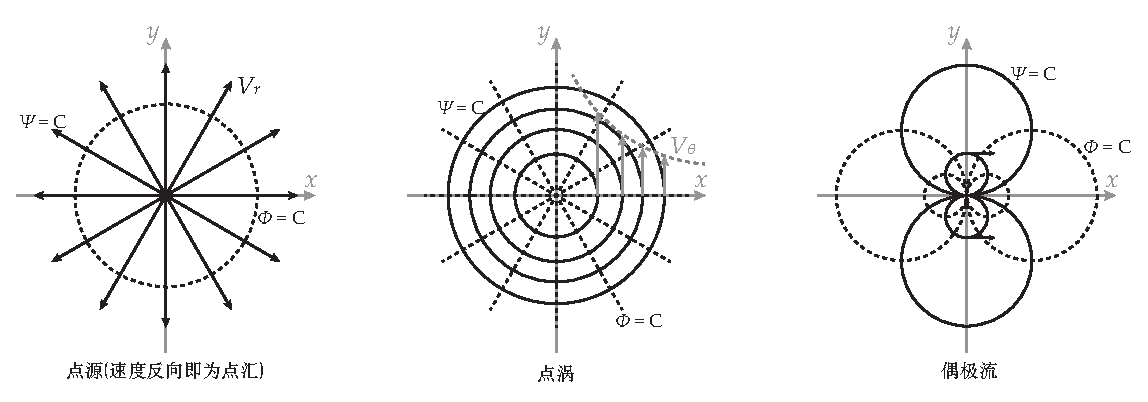
\includegraphics[scale=0.6]{figures/点源点涡偶极流.eps}
	\caption{点源、点涡和偶极流的流线和等势线}
\end{figure}

\LevelTwoTitle{*圆柱绕流}

\LevelThreeTitle{无环量圆柱绕流}

由$\vec{x}$方向均匀来流和$-\vec{x}$方向偶极流叠加而成,圆柱表面速度分布

\begin{align*}
	&V_r = 0\\
	&V_{\theta} = -2U \sin \theta 
\end{align*}

\begin{enumerate}
	\item $\theta = 0, \pi$,驻点;
	\item $\theta = \pm \dfrac{\pi}{2}$,舷点。
\end{enumerate}

\begin{figure}[H]
	\centering
	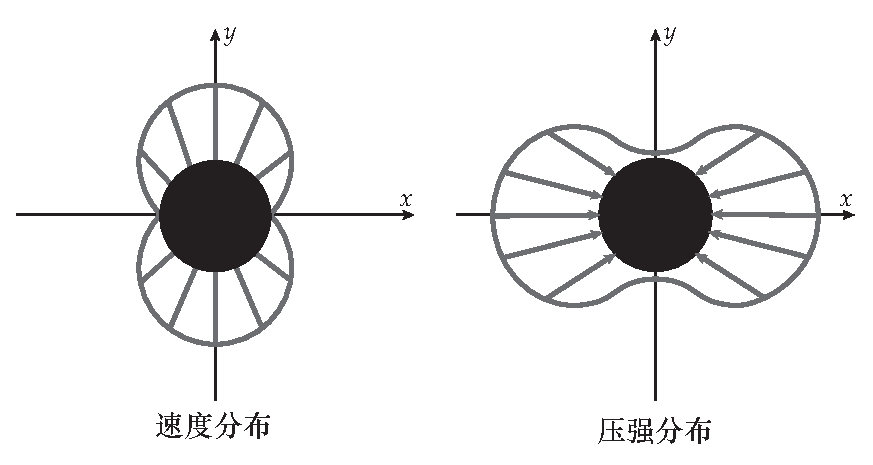
\includegraphics[scale=0.7]{figures/无环量.eps}
	\caption{无环量圆柱绕流的速度分布和压强分布}
\end{figure}

\LevelThreeTitle{有环量圆柱绕流}

由无环量圆柱绕流和点涡叠加而成,圆柱表面速度分布

\begin{align*}
	&V_r = 0\\
	&V_{\theta} = -2U \sin \theta \pm \dfrac{\varGamma}{2\pi R}
\end{align*}

$V_{\theta}$第二项,顺时针取负,逆时针取正。令其等于零,得驻点表达式$\sin \theta_s = \pm \dfrac{\varGamma}{4\pi R U}$,关于驻点个数讨论如下

\begin{enumerate}
	\item $\varGamma < 4\pi R U$,2个;
	\item $\varGamma = 4\pi R U$,1个;
	\item $\varGamma > 4\pi R U$,0个。
\end{enumerate}

\begin{figure}[H]
	\centering
	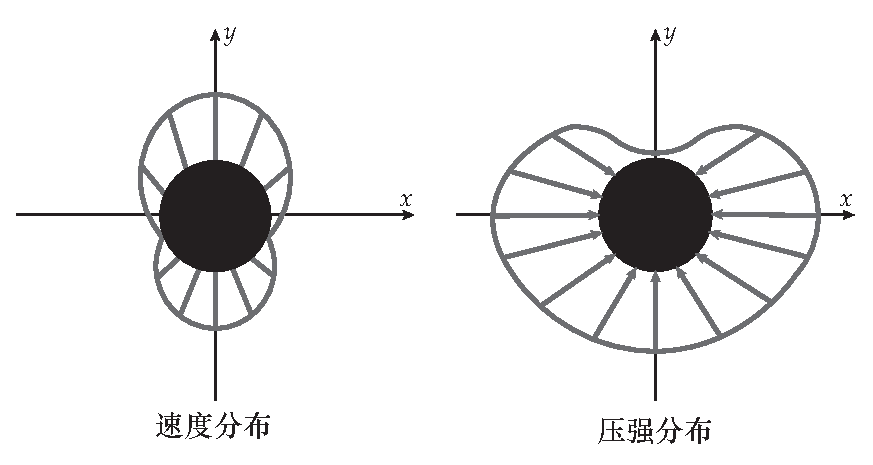
\includegraphics[scale=0.7]{figures/有环量.eps}
	\caption{有环量圆柱绕流的速度分布和压强分布}
\end{figure}

\LevelThreeTitle{达朗贝尔悖论}

理想不可压缩流动中任一封闭物体绕流阻力为零,产生此悖论的原因是没有考虑粘性。

\LevelTwoTitle{例题练习}

\begin{example}
	试证明$\psi = x + 2x^2 - 2y^2$所表示的流动是势流,并求出该流动的速度势函数。若流体的密度是1.21 kg/m$^3$,在点$(1, -2)$处压强$p = 4.8$ kPa,试求点$(9, 6)$处的压强。
	
	\begin{equation*}
		\nabla^2 \psi = \pdv[2]{\psi}{x} + \pdv[2]{\psi}{y} = 4 - 4 = 0
	\end{equation*}
    故该流动是势流。
    \begin{equation*}
    	u = \pdv{\psi}{y} = \pdv{\phi}{x} = -4y, ~v = -\pdv{\psi}{x} = \pdv{\phi}{y} = -1 - 4x
    \end{equation*}
    于是
    \begin{equation*}
    	\phi = \int -4y \dd{x} + f(y) = -4xy + f(y)
    \end{equation*}
    求导
    \begin{equation*}
    	\pdv{\phi}{y} = -4x + f'(y) = v
    \end{equation*}
    对比,得
    \begin{equation*}
    	f'(y) = -1 \Rightarrow f(y) = -y + C
    \end{equation*}
    故$\phi = -4xy - y + C$。
    速度分布
    \begin{equation*}
    	\vec{V} = u \vec{i} + v \vec{j}
    \end{equation*}
    则$(1, -2)$点处$V_1^2 = 89 \mathrm{~m}^2 / \mathrm{s}^2$,$(9, 6)$点处$V_2^2 = 1945 \mathrm{~m}^2 / \mathrm{s}^2$。
    
    列伯努利方程
    \begin{equation*}
    	\dfrac{p_1}{\rho} + \dfrac{V_1^2}{2} = \dfrac{p_2}{\rho} + \dfrac{V_2^2}{2}
    \end{equation*}
    解得
    \begin{equation*}
    	p_2 = 3.76 \mathrm{~kPa}
    \end{equation*}
\end{example}

\begin{tip}
	2021年计算题第一道跟本题类似,需要对速度、速度势函数和流函数之间的关系很清楚。叠加类题目考的概率比较小,若要练习可以参考课后题8.13 ~ 8.21。
\end{tip}
